\documentclass{article}

\usepackage[utf8]{inputenc}
\usepackage[T1]{fontenc}
\usepackage{microtype}

\usepackage{newspaper}
%% [LianTze] Contains some modifications
\usepackage{newspaper-mod}
%%... so now you can redefine the headline and byline style if you want to.
%% These can be issued just before any
%% byline or headline in the paper, to
%% individually style each article
%%
% \renewcommand{\headlinestyle}{\itshape\Large\lsstyle}
% \renewcommand{\bylinestyle}{\bfseries\Large\raggedright}


\date{\today}
\currentvolume{1}
\currentissue{5}

%% [LianTze] The newspaper package also provides 
%% these commands to set various metadata:

%% The banner headline on the first page
%%   (The colon after s: is to get a more
%%   modern majuscule s in this font instead of 
%%   the medieval tall s. For anyone interested 
%%   in the history: 
%%  http://medievalwriting.50megs.com/scripts/letters/historys.htm)
\SetPaperName{Liberty City Outsider}

%% The name used in the running header after
%% the first page
\SetHeaderName{Transformation news}

%% and also...
\SetPaperLocation{The Guild}
\SetPaperSlogan{Первый просветительский выпуск}
\SetPaperPrice{Free}


% [LianTze] times (the package not the font) is rather outdated now; use newtx (see later)
% \usepackage{times}
\usepackage{graphicx}
\usepackage{wrapfig}
\usepackage{multicol}

\usepackage{picinpar}
%uasage of picinpar:
%\begin{window}[1,l,\includegraphics{},caption]xxxxx\end{window}


%%%%%%%%%  Front matter   %%%%%%%%%%

\usepackage{lipsum}

\begin{document}

\maketitle

\begin{multicols}{3}

\headline{\bf\sf\Large Собираем колоду}
Готовим срочный выпуск. Требование от бизнеса.
\\\\Подробности на странице 2 >>
\vspace{20mm}
\closearticle

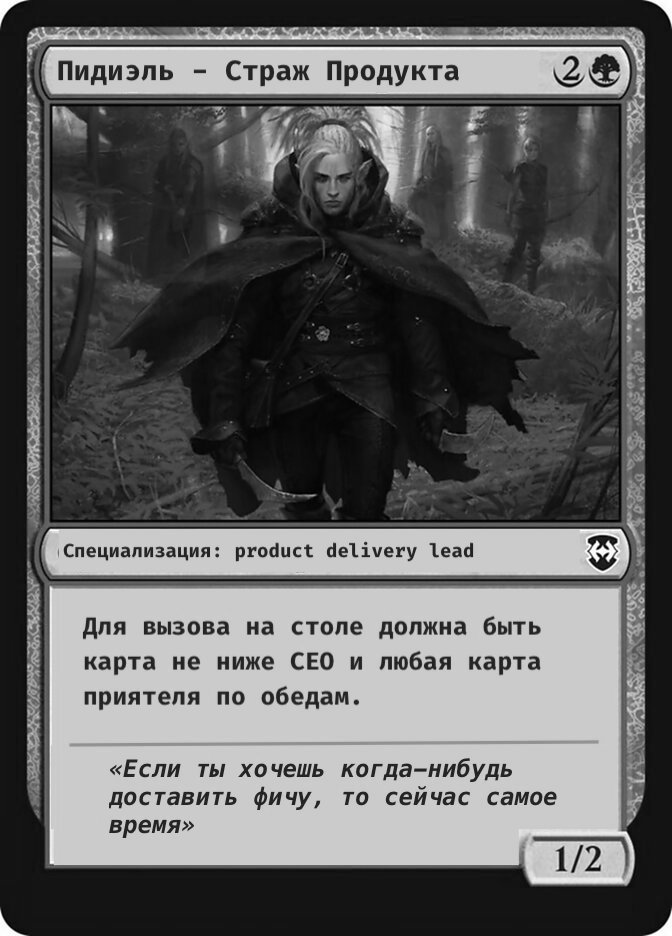
\includegraphics[width=11.2cm]{main.jpeg}

\end{multicols}

\begin{multicols}{3}

\headline{\bf\sf\Large Люди-ботлнеки}
Что будет без них - где подавимся, а где захлебнёмся?
\\\\Подробности на странице 2 >>
\vspace{8mm}
\closearticle

\headline{\bf\sf\Large Как съесть слона}
Жопа в начале или жопа в конце? Расставим приоритеты и нарисуем роудмап на странице 3 >>
\vspace{10mm}
\closearticle

\headline{\bf\sf\Large Not MVP}
Пока ничего не делаем на странице 3 >>
\vspace{8mm}
\closearticle

\end{multicols}

\end{document}